 \documentclass[class=report,crop=false, 12pt]{standalone}
\usepackage[screen]{../scratch}

\begin{document}


\titre[E]{Listes}
%===============================


\begin{enigme}

On pose $3$ masses sur une plaque triangulaire.
En $A$ et $B$ chaque masse est de $1$ kg, en $C$ elle est de $2$ kg.


\myfigure{0.8}{
\tikzinput{triangle}
}  


Les coordonnées $[x_A,y_A,x_B,y_B,x_C,y_C]$ de $A$, $B$, $C$ sont données par la liste :
$$[20,50,0,150,150,100].$$

Le \emph{centre de gravité} $G$ a pour coordonnées :
$$x_G = \frac{x_A+x_B+2x_C}{4}$$
$$y_G = \frac{y_A+y_B+2y_C}{4}$$


\bigskip

\textbf{Question.} Calcule les coordonnées $(x_G,y_G)$. 
Combien vaut $x_G+y_G$ ?
 

%\begin{solution}
%$x_G = 80$, $y_G = 100$. Réponse : $180$.
%\end{solution}

\end{enigme}



\begin{enigme}
Un mot ou une phrase est une suite de caractères et se comporte à peu près comme une liste. Les éléments de la liste étant les caractères.


Voici un programme.

\begin{center}
  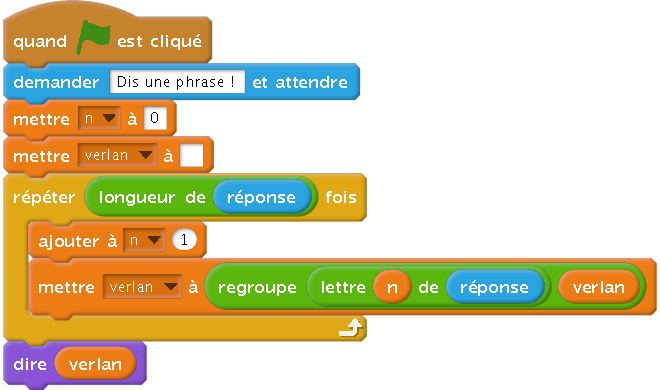
\includegraphics[scale=\scalebloc,scale=0.7]{code-12-eg2}   
\end{center}


\bigskip

\textbf{Question.} Lorsque l'ordinateur interroge l'utilisateur, celui-ci tape le mot \og Bonjour \fg{}. Que dit alors Scratch ?

%\begin{solution}
%Les lettres sont inversées : \og ruojnoB \fg{}.
%\end{solution}

\end{enigme}


\begin{enigme}

\sauteligne

\begin{itemize}
  \item Une urne contient $6$ boules : 3 noires, 2 rouges, 1 bleue.
  \item On tire au hasard une première boule, \emph{mais on ne la remet pas dans l'urne}.
  \item On tire au hasard un seconde boule.
  \item C'est gagné si l'une des boules est rouge et que l'autre est bleue.
\end{itemize}

\bigskip

\emph{Indication.} Deux possibilités pour modéliser un tirage sans remise : 
\begin{enumerate}
  \item Tirer la première boule. Supprimer la première boule de la liste. Puis tirer la seconde boule.
  
  \item Tirer deux nombres $n_1$ et $n_2$ au hasard entre $1$ et $6$ jusqu'à ce qu'ils soient différents. La première boule sera l'élément $n_1$ de la liste et la seconde l'élément $n_2$.
\end{enumerate}
  

\bigskip

\textbf{Question.} Sur $10\,000$ tirages, combien d'entre eux environ sont gagnants ?
Donne la réponse parmi les entiers :
$100$, $300$, $500$, $700$, $900$, $1100$, $1300$, $1500$...


%\begin{solution}
%Environ $1300$.
%\end{solution}

\end{enigme}

\end{document}

